\section*{Introduction}
The proposed solutions for attendance both involve the use of face recognition/detection technologies. 
\newline
The first solution suggests mapping faces to seats. In this solution, each student's face would be detected and mapped to their seat in the classroom. During each lecture, the system would capture an image of the classroom and compare it to the mapped faces. If a face is present at a particular seat, the system would assume that the person occupying the seat is the student mapped to that face and mark their attendance.
\newline
The second solution is more computation-heavy but offers more accurate attendance tracking. In this solution, each student's face would be recognized individually, and their attendance would be marked based on their presence in the classroom. The system would capture an image of the classroom and identify each individual face, matching it to the faces of students enrolled in the class. Once a face is recognized, the attendance of the corresponding student would be marked as present. This approach would require more processing power and storage capacity to store and compare each individual face, but it would provide more accurate attendance tracking and prevent errors that may occur with the mapping of faces to seats approach.

\section{Face Detection / Mapping Method}
\subsection{Preprocessing}
An empty image of the lecture hall is captured to identify the seating arrangement, and a list or mapping of students with their corresponding seats is created. This enables us to accurately map the detected faces to their respective seats during attendance taking.
\subsection{Detection Algorithm}
Various algorithms such as HOG+SVM, MTCNN, and Harcascade are used for face detection. These algorithms analyze the input image to identify regions containing human faces. Upon detection, the face's location is represented by its $(x,y)$ coordinates within the image, which are further processed to provide an accurate positional representation in subsequent steps.

\subsection{Mapping coordinates}
The process of mapping a person to a seat involves comparing the coordinates $(x,y)$ of the detected face with the coordinates $(x_i,y_i)$ of the seats in the lecture hall. If the absolute difference between the x-coordinates of the detected face and the seat is less than a certain threshold value and the absolute difference between the y-coordinates of the detected face and the seat is also less than the same threshold value, then the person is considered to be seated at that particular seat. The threshold value determines how close the detected face needs to be to the actual seat coordinates for the mapping to occur.
\newline
\begin{equation}
    |\text{x}-\text{x}_i| \leq \delta  \;\; \& \;\; |\text{y}-\text{y}_i| \leq \delta
\end{equation}
Here the $\delta$ is also dependent on the $(x,y)$ as we go up the image the $\delta$ keeps decreasing .

\clearpage
\section{Face Recognition / Identification Method}
\subsection{Preprocessing}
In order to perform face recognition using a Convolutional Neural Network (CNN), we need to have a database of students enrolled in the class. For each student, we extract distinct features of their face and map them to a vector of size 128 bits using a feature extraction algorithm. This vector is then stored in the database along with the student's name and other relevant information.
Having a database of students and their corresponding feature vectors is crucial for accurate recognition and attendance marking using a CNN-based approach.

\subsection{Data Streaming}
To use an IP camera for face recognition, the first step involves establishing a network connection with the camera and retrieving its video stream. This video stream is then analyzed frame by frame to detect any faces present in the stream. This is achieved by applying a face detection algorithm such as DLIB CNN to each frame of the video.

Once a face is detected, the face recognition algorithm is used to extract 128-dimensional feature vectors from the face. These vectors are then compared to the vectors of previously enrolled students in the database to recognize them.

This process is repeated for each frame of the video stream, allowing the system to mark the attendance of recognized students. However, this process can be computationally intensive, especially when dealing with high-resolution video streams. To ensure real-time processing, specialized hardware or algorithm optimization may be required.

\subsection{Recognition}
Dlib-based face recognition uses a Convolutional Neural Network (CNN) to extract features from a face image. The features are stored in a 128-dimensional vector called the 128-bit vector. To recognize a face, the CNN first detects and aligns the face in the input image. Then, it extracts 128 features and compares them to the vectors of enrolled students using the Euclidean distance metric. If the distance is below a certain threshold, the face is considered a match, and attendance is marked. The threshold is adjustable and depends on the application's specific requirements.

\begin{figure}[!htb]
    \centering
    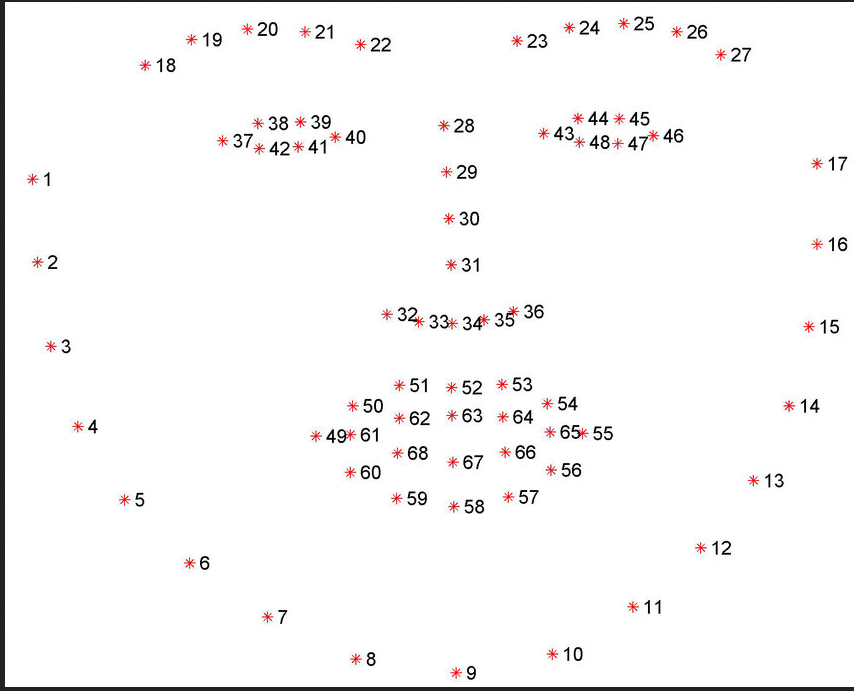
\includegraphics[width=\linewidth,height=0.8\linewidth]{Figures/Ch01/128bit.png}
    \caption{cascade}
    \label{figure:cascade}
    \end{figure}

\section{Marking attendance}
Once a face is recognized and matched to a student in the database, their attendance can be marked as present. This is usually done by updating a record in a database or spreadsheet with the student's name, timestamp, and any other relevant information.